% Arquivo Principal para Dissertações do PPGCA - Udesc Joinville

% abnTeX2: Modelo de Trabalho Academico em conformidade com
% ABNT NBR 14724:2011: Informacao e documentacao - Trabalhos academicos -
% Apresentacao

% Adaptado com base no abnTeX2
% Por: Luís Felipe Bilecki
% E-mail: luis.bilecki@gmail.com
% ------------------------------------------------------------------------
% ------------------------------------------------------------------------
\documentclass[
	12pt,				% tamanho da fonte
	openright,			% capítulos começam em pág ímpar (insere página vazia caso preciso)
	oneside,
	a4paper,			% tamanho do papel.
	chapter=TITLE,		% títulos de capítulos convertidos em letras maiúsculas
	section=TITLE,		% títulos de seções convertidos em letras maiúsculas
	%subsection=TITLE,	% títulos de subseções convertidos em letras maiúsculas
	%subsubsection=TITLE,% títulos de subsubseções convertidos em letras maiúsculas
	% -- opções do pacote babel --
	english,			% idioma adicional para hifenização
	brazil,				% o último idioma é o principal do documento
	]{abntex2}

%Pacotes prinicipais e customização
\usepackage{./Estilo/udesc}

% ---
% Dados da Capa
% ---

\titulo{SISTEMA DE RECOMENDAÇÃO SENSÍVEL AO TEMPO EM AMBIENTES VIRTUAIS DE APRENDIZAGEM}
\autor{EDUARDO JOSÉ DE BORBA}
\local{Joinville}
\instituicao{Universidade do Estado de Santa Catarina - UDESC}
\campus{Centro de Ciências Tecnológicas - CCT}
\curso{Mestrado em Computação Aplicada}
\data{2017}
\fulldata{11 de Dezembro de 2017}

% ---
% Folha de Rosto
% ---
\inforosto{Qualificação apresentada ao Programa de Pós-Graduação em Computação Aplicada, da Universidade do Estado de Santa Catarina, como requisito parcial para a obtenção do grau de Mestre em Computação Aplicada.}
\orientador{Isabela Gasparini}
\orientadorRotulo{Dra. }
\coorientador{Daniel Lichtnow}
\coorientadorRotulo{Dr. }

% ----
% Início do documento
% ----
\begin{document}
% ----
% Elementos Pré-Textuais
% ----
%!TEX root = ../Principal.tex
%Capa do Trabalho
\imprimircapa

%Folha de Rosto
%* indica que tem ficha catalográfica
\imprimirfolhaderosto*

% ---
% Caso a Biblioteca da UDESC forneça, utilize o comando
% ---
% \begin{fichacatalografica}
%     \includepdf{fig_ficha_catalografica.pdf}
% \end{fichacatalografica}

% ---
% Geração da Ficha Catalográfica Via LaTeX
% ---
% \begin{fichacatalografica}
% 	\vspace*{\fill}					% Posição vertical
% 	\begin{center}					% Minipage Centralizado
% 	\begin{minipage}[c]{12.5cm}		% Largura

% 	\imprimirautor

% 	\hspace{0.5cm} \imprimirtitulo  / \imprimirautor. --
% 	\imprimirlocal, \imprimirdata-

% 	\hspace{0.5cm} \pageref{LastPage} p. : il. (algumas color.) ; 30 cm.\\

% 	\hspace{0.5cm} \imprimirorientadorRotulo~\imprimirorientador\\

% 	\hspace{0.5cm}
% 	\parbox[t]{\textwidth}{\imprimirtipotrabalho~--~\imprimirinstituicao,
% 	\imprimirdata.}\\

% 	\hspace{0.5cm}
% 		1. Tópico 01.
% 		2. Tópico 02.
% 		I. Prof. Dr. xxxxx.
% 		II. Universidade do Estado de Santa Catarina.
% 		III. Centro de Ciências Tecnológicas.
% 		IV. identificação xxxx\\

% 	\hspace{8.75cm} CDU 02:121:005.7\\

% 	\end{minipage}
% 	\end{center}
% \end{fichacatalografica}

% % ---
% % Folha de Aprovação
% % ---
% % Exemplo de folha de aprovação antes da Banca. Após isso, incluia o pdf digitalizado com as assinaturas%
% % 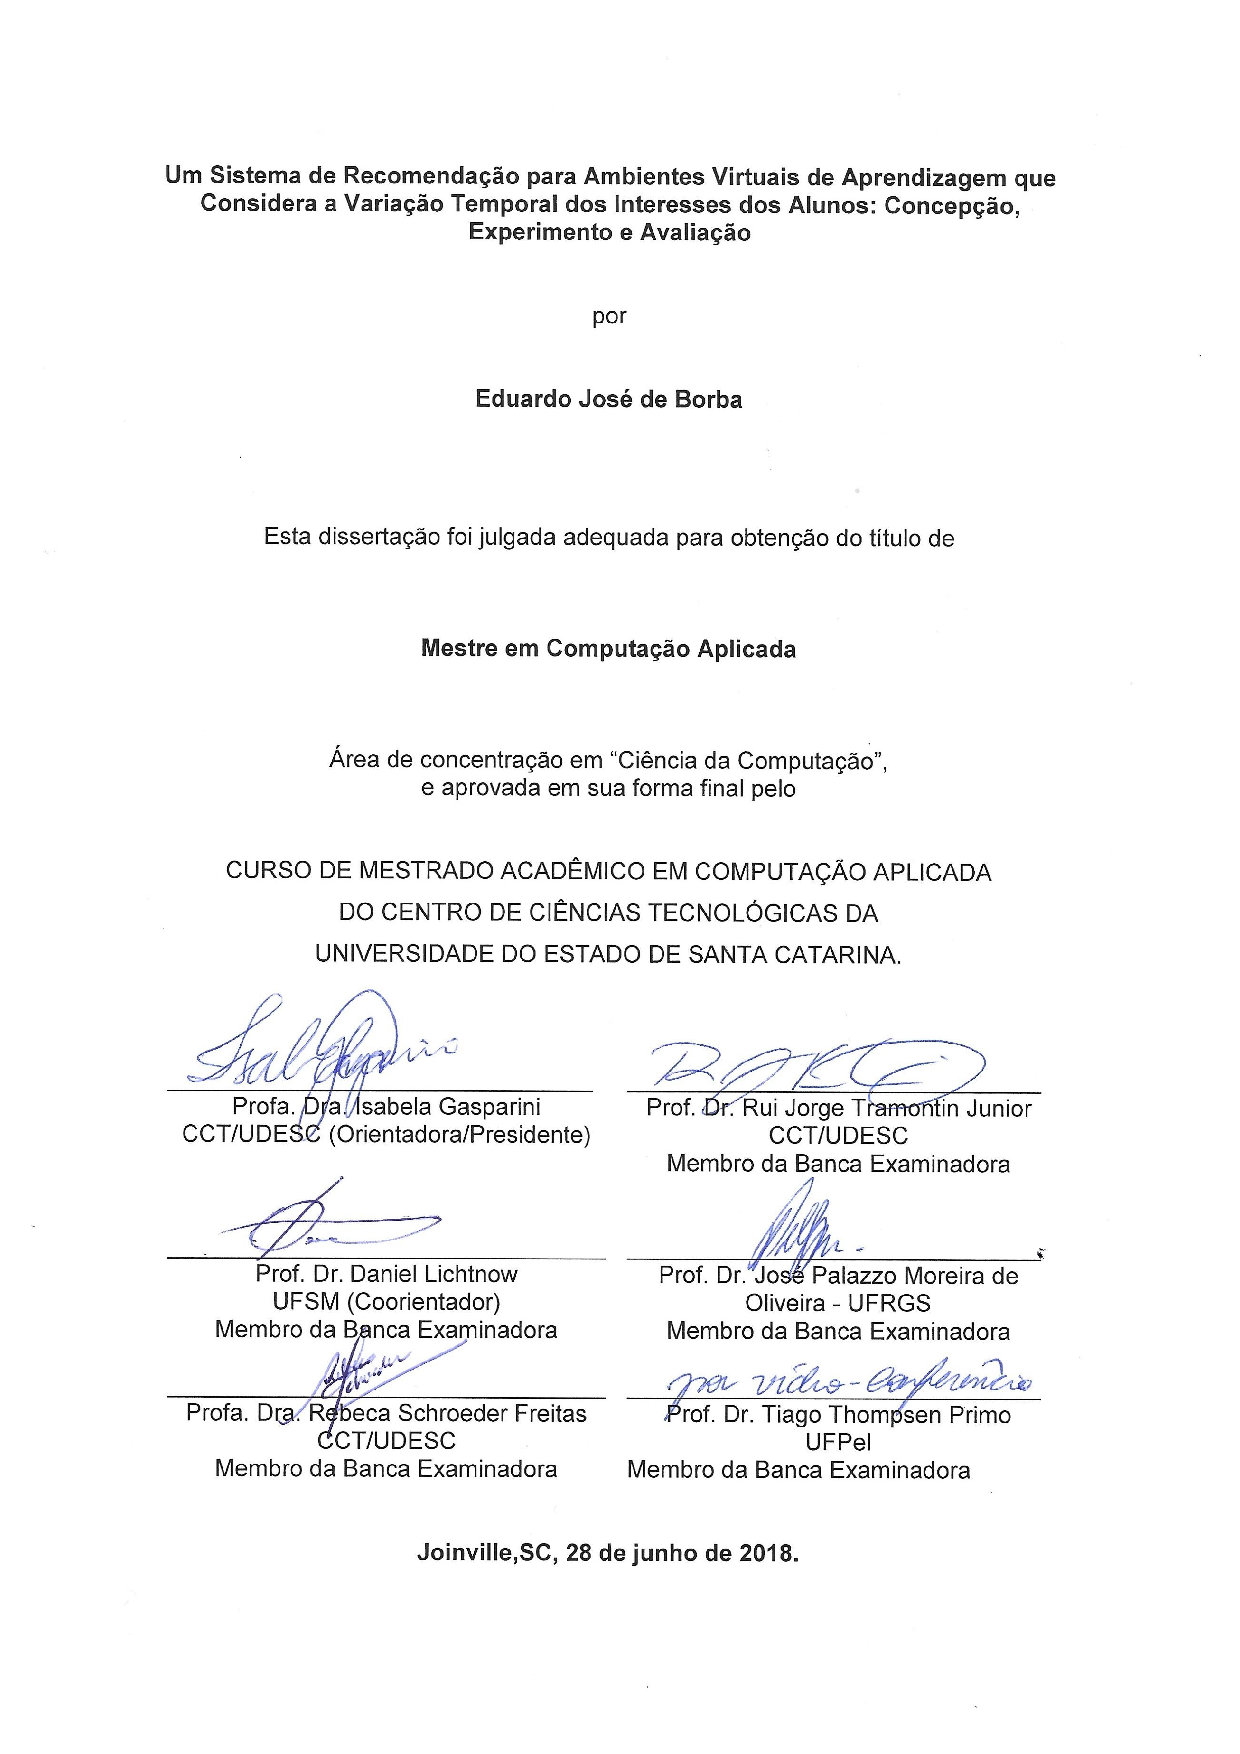
\includepdf{folhadeaprovacao_final.pdf}
\begin{folhadeaprovacao}
	\begin{center}
		{\ABNTEXchapterfont\bfseries\imprimirautor}
		\vspace{2em}

			\ABNTEXchapterfont\bfseries\imprimirtitulo

	\end{center}
		\vspace{1em}
		{\justify
    Dissertação apresentada ao Programa de Pós-Graduação em Computação Aplicada, da Universidade do Estado de Santa
    Catarina, como requisito parcial para a obtenção do grau de Mestre em Computação Aplicada.}
	 \vspace{2em}
	\noindent

	{\justify \bfseries Banca Examinadora}

  \vspace{2em}

  \noindent{Orientadora:\hfill \assinatura*{\textbf{\imprimirorientadorRotulo \imprimirorientador} \\ Universidade do Estado de Santa Catarina (UDESC)}}

  \noindent{Coorientador:\hfill \assinatura*{\textbf{\imprimircoorientadorRotulo \imprimircoorientador} \\ Universidade Federal de Santa Marina (UFSM)}}

  \noindent{Membros:}

	\noindent{\assinatura*{\textbf{Dr. Rui Jorge Tramontin Junior} \\ Universidade do Estado de Santa Catarina (UDESC)}}
  \noindent{\assinatura*{\textbf{Dra. Rebeca Schroeder Freitas} \\ Universidade do Estado de Santa Catarina (UDESC)}}
  \noindent{\assinatura*{\textbf{Dr. Thiago T. Primo} \\ Universidade Federal de Pelotas (UFPel)}}
  \noindent{\assinatura*{\textbf{Dr. José Palazzo M. de Oliveira} \\ Universidade Federal do Rio Grande do Sul (UFRGS)}}

    \vspace*{\fill}
    \begin{center}
    	\imprimirlocal,\,\imprimirfulldata
    \end{center}
\end{folhadeaprovacao}

% ---
% Dedicatória
% ---
% \begin{dedicatoria}
% Dedico este trabalho aos meus familiares, amigos, colegas e professores que me acompanharam e me deram forças nessa magnífica trajetória.
% \end{dedicatoria}

% % ---
% % Agradecimentos
% % ---
% \begin{agradecimentos}
% Gostaria de agradecer...

% Aqui devem ser colocadas os agradecimentos às pessoas que de alguma forma contribuíram para a realização do trabalho.
% \end{agradecimentos}

% ---
% Epígrafe
% ---
% \begin{epigrafe}
% ``Independentemente das circunstâncias, devemos ser sempre humildes, recatados e despidos de orgulho.''
% \\
% \par
% Dalai Lama
% \end{epigrafe}

% ---
% RESUMOS
% ---

% Português
\begin{resumo}
  Sistemas de Recomendação (SR) são ferramentas de software que sugerem itens para os usuários de forma automatizada e personalizada,
  sem a necessidade do usuário formular uma consulta para encontrar os itens do seu interesse. Esses sistemas são
  explorados em Ambientes Virtuais de Aprendizagem (AVA) com o objetivo de reduzir alguns problemas existentes nesses ambientes
  quando a quantidade de materiais disponíveis é grande, tais como: sobrecarga cognitiva, dificuldade de encontrar os materiais
  do seu interesse e muitos materiais nunca serem utilizados. Pesquisadores da área argumentam que os algoritmos de SRs tradicionais não são suficientes para os AVAs,
  sendo necessário um nível maior de personalização a situação do usuário, como considerar dimensões do contexto. O objetivo
  desse trabalho é a criação de perfis de usuário que levem em conta a mudança dos interesses destes usuários
  ao longo do tempo. O algoritmo proposto combina a (1) similaridade do perfil do usuário (representado
  pelos materiais acessados pelo usuário) com os itens disponíveis para a recomendação com a (2) recência do acesso ou uso
  desse materiais, além da (3) informação se aquele item disponível para a recomendação já foi acessado ou não. A
  proposta leva em conta que o ritmo de estudo dos alunos pode ser diferente, portanto a recência é considerada em relação
  a sequência de itens acessados e não ao tempo absoluto (em segundos) desde o acesso. A proposta desse trabalho será
  incorporada ao ambiente \adaptweb e será avaliado através de um minicurso de algoritmos ministrado no ambiente.
  O algoritmo proposto será comparado a abordagem Baseada em Conteúdo tradicional através de um experimento utilizando um
  estratégia \textit{Between Subjects}. O objetivo do experimento é verificar se existe diferença na percepção do usuário
  sobre a qualidade das recomendações do algoritmo proposto em relação a abordagem Baseada em Conteúdo tradicional.

  \vspace{\onelineskip}

  \noindent
  \textbf{Palavras-chaves}: Sistema de Recomendação; Sensível ao Tempo; Sensível ao Contexto; Ambiente Virtual de Aprendizagem; \adaptweb.
\end{resumo}

% Inglês
\begin{resumo}[Abstract]
 \begin{otherlanguage*}{english}
  	Recommender Systems (RS) are software tools that provide items as suggestions to users automatically and personalized to his
    interests, without the need to formulate a search argument to achieve this. This systems are applied to Virtual Learning
    Environments (VLE) aiming to reduce some drawbacks existing in this enviroments when the number of available items is
    huge, e.g., cognitive overload, difficulty finding items of user's interest or some materials never get used. Researchers
    in this area argues that traditional RS approaches are not enough for VLE, being required a major level of personalization
    to user's current context. This work goals is to create user profiles that take into account the changing of user's interests
    with the time. This profiles are going to be applied in the recommendation algorithm proposed in this work. The proposed
    algorithm combines (1) similarity between user profile (represented by materials accessed by the user) with the items
    available to recommendation with (2) the recency of materials accessed by the user and (3) the information about if
    the item available to be recommended were accessed or not. The proposal takes into account that each learner can have
    a different study rhythm, therefore the recency considers the sequence of items accessed and not the absolute time (in
    seconds) from the access. The proposal of this work will be incorporate to the \adaptweb environment and will be evaluated
    through an algorithms course in the environment. The proposal will be compared to the Content-Based traditional approach
    through an experiment using a Between Subjects strategy. The objective of this experiment is to verify if exists differences
    in user's perception of quality recommendations between the proposal when compared with Content-Based approach.
    \vspace{\onelineskip}

    \noindent
    \textbf{Keywords}: Recommender System; Time-Aware; Context-Aware; Virtual Learning Environment; \adaptweb.
 \end{otherlanguage*}
\end{resumo}

% ---
% Lista de Figuras
% ---
\pdfbookmark[0]{\listfigurename}{lof}
\listoffigures*
\cleardoublepage
% ---

% ---
% Lista de Tabelas
% ---
\pdfbookmark[0]{\listtablename}{lot}
\listoftables*
\cleardoublepage

% ---
% Lista de Abreviaturas e Siglas
% ---
\begin{siglas}
  \SingleSpacing
  \item[AdaptWeb\textsuperscript{\textregistered}]  Ambiente de Ensino-Aprendizagem Adaptativo na Web
  \item[AVA]       Ambiente Virtual de Aprendizagem
  \item[CCT]       Centro de Ciências Tecnológicas
  \item[PPGCA]     Programa de Pós-Graduação em Computação Aplicada
  \item[SR]        Sistema de Recomendação
  \item[TCLE]      Termo de Consentimento Livre e Esclarecido
  \item[UDESC]     Universidade do Estado de Santa Catarina
  \item[UFRGS]     Universidade Federal do Rio Grande do Sul
  \item[UFSM]      Universidade Federal de Santa Maria
  \item[XML]       Extensible Markup Language
\end{siglas}

% ---
% inserir o sumario
% ---

\pdfbookmark[0]{\contentsname}{toc}
\tableofcontents*
\cleardoublepage
% ---

\textual

%Retira o nome do capítulo do header
\pagestyle{eudesc}
\aliaspagestyle{chapter}{eudesc}

% ---

\chapter{Introdução}\label{introducao}

\section{Objetivos}

Foram definidos objetivos geral e específicos para orientar o processo de pesquisa desse trabalho.

\subsection{Objetivo Geral}

Considerando sistemas de recomendação voltados para ambientes de aprendizagem, criar modelos de usuário que levem em
conta a mudança dos interesses destes usuários ao longo do tempo.

\subsection{Objetivos Específicos}

\begin{itemize}
\item Definir algumas formas de levar em conta aspectos temporais em um algoritmo de recomendação
\item Definir como usar o aspecto temporal em sistemas de recomendação para ambiente educacionais
\item Implementar o algoritmo de recomendação proposto no ambiente AdaptWeb\textsuperscript{\textregistered}
\item Considerar diretrizes de apresentação de recomendação ao desenvolver a interface do sistema de recomendação
no ambiente AdaptWeb\textsuperscript{\textregistered}
\item Avaliar a qualidade de uso do sistema de recomendação proposto pela perspectiva do usuário
\end{itemize}

\section{Escopo}

Esse trabalho não irá considerar outras dimensões do contexto além do tempo na recomendação, e dentro do uso do contexto
temporal apenas a categoria de \textit{Decay} será aplicada nesse trabalho. Além disso, a única abordagem de recomendação
utilizada será a Baseada em Conteúdo, apesar de as categorias de Sistemas de Recomendação Sensíveis ao Tempo poderem ser
aplicadas em quaisquer abordagens de recomendação. A avaliação do Sistema de Recomendação proposto será feita apenas em ambientes educacionais, mesmo sendo
possível aplicá-lo em outros domínios de aplicação. Não será avaliado, nesse trabalho, o impacto da proposta na aprendizagem
dos alunos.

\section{Metodologia}

\section{Estrutura}




\chapter{Fundamentação Teórica}

\section{Sistemas de Recomendação}

Sistemas de Recomendação (SRs) se tornaram uma importante área de pesquisa a partir dos anos 90, quando começaram a
surgir os primeiros trabalhos na área de filtragem colaborativa \cite{adomavicius2005toward}. Os SRs são ferramentas
computacionais que provém sugestões de itens personalizadas aos usuários \cite{ricci2011introduction}. Isso significa
que o usuário recebe um como recomendaçnos um conjunto diferente de itens de acordo com as suas preferências e necessidades.
Nos últimos anos, o interesse na aplicação de SRs têm crescido fortemente \cite{adomavicius2005toward, beel2016towards}.
Exemplos dessas aplicações são: recomendação de Livros, CDs, DVDs, etc., em sites de e-commerce como Amazon e EBAY;
recomendações de filmes em sites como MovieLens e Netflix; recomendação de músicas em sites de streaming como Last.fm ou
Spotify; recomendação de amigos ou de postagens em redes sociais como Facebook ou Twitter.

SRs podem ser presentados formalmente como:

Onde F é a função que busca prever o interesse do usuário pelos itens existentes, U representa o conjunto dos usuários,
I representa o conjunto dos itens e R representa a lista ordenada dos itens pelo interesse previsto para o usuário ativo
(o usuário que irá receber a recomendação). O objetivo do SR então é conseguir prever de maneira mais correta, com as
informações disponíveis, os itens que serão de maior interesse do usuário.

Existem duas formas de capturar os interesses do usuário pelos itens acessados dentro do sistema: (1) Explicita, na
qual o usuário indica explicitamente o seu interesse pelo item que acabou de acessar, geralmente com uma nota 1 a 5 ou
apenas uma indicação de interesse positivo/negativo para o item; (2) Implícita, na qual o usuário não precisa indicar o
seu interesse pelo item, essa informação é capturada implicitamente através do seu comportamento e das suas interações
dentro do sistema.

Os SRs podem ser classificados de acordo com a forma como as recomendações são realizadas (abordagem). As principais
abordagens citadas na literatura são \cite{torres2004personalizaccao, adomavicius2005toward, ricci2011introduction}:
Baseada em Conteúdo, Filtragem Colaborativa, Baseada em Conhecimento e Híbrida. Nas subseções a seguir são descritas
cada uma dessas abordagens.

\subsection{Baseada em Conteúdo}

Segundo \citeonline{ricci2011introduction}, essa é uma abordagem na qual o usuário recebe recomendações de itens
similares aos que se interessou no passado. Consiste em avaliar a semelhança entre um item e os interesses do usuário.
Utilizando a nomenclatura utilizada por \citeonline{adomavicius2005toward}, os métodos dessa abordagem tentam prever o
grau de utilidade de um item para um usuário com base na utilidade que o usuário determinou para os itens similares ao item.

A abordagem Baseada em Conteúdo tem suas raízes na Recuperação da Informação \cite{adomavicius2005toward}. Para a
abordagem Baseada em Conteúdo, teremos um conjunto de atributos descrevendo um item e um conjunto de atributos
descrevendo os gostos e preferências do usuário. A descrição de um item frequentemente é realizada através de
palavras-chave definidas automaticamente por meio de algoritmos usados na área de Recuperação da Informação
\cite{adomavicius2005}. Já a descrição das preferências do usuário pode ser capturada de duas formas: implícita,
através do seu comportamento no ambiente e de itens que acessou; ou explícita, onde o usuário informa suas preferências
ao sistema, por exemplo, respondendo a questionários (ADOMAVICIUS e TUZHILIN, 2005). Dessa forma, os SRs de itens
textuais (e.g., documentos) são os que mais utilizam a abordagem Baseada em Conteúdo, devido à facilidade da aplicação
das técnicas de Recuperação da Informação nesse tipo de item.

Dentro da área de Recuperação da Informação uma forma de medir a similaridade de itens em um SR é o Cosseno. O cálculo da similaridade por Cosseno foi definido por Salton nos anos 60 (SALTON, 1964). Nessa técnica, cada documento é representado por um vetor de termos . Os vetores são dispostos em um espaço vetorial de  dimensões, onde  é o número de termos, e documentos próximos nesse espaço são considerados semelhantes. Para verificar essa proximidade utiliza-se a seguinte fórmula (MANNING et al., 2009):

Onde:  é o resultado da distância dos vetores, variando de [0,1];  é o termo presente na posição  do item 1; é o termo presente na posição  do item 2. Por exemplo, se tivermos três vetores:  representado o usuário,  e representando itens. Ao calcular a similaridade entre esses itens, temos  e , identificando que o item representado por  é mais similar às preferências do usuário c.
Outra técnica de Recuperação da Informação é o tf-idf (term-frequency inverse document frequency). Essa técnica é utilizada para identificar termos importantes em um documento (MANNING et al., 2009) e pode ser utilizada para a descoberta das palavras-chave que descrevem um item. É utilizada a seguinte fórmula para o cálculo dos pesos de cada termo do documento (MANNING et al., 2009):

Onde: representa o peso do termo  no documento ;  é o número de vezes que o termo  aparece no documento ; e o  representa o Inverse document frequency do termo , sendo o responsável por identificar termos que aparecem em muitos documentos diferentes (MANNING et al., 2009). Os termos que aparecem em muitos documentos tendem a perder sua importância. O  é calculado através da seguinte fórmula (MANNING et al., 2009):

Onde:  é o número total de documentos em uma coleção; e  é o número de documentos onde aparece o termo .
A principal vantagem da abordagem Baseada em Conteúdo é não necessitar da opinião de outros usuários para a recomendação (RICCI et al., 2011). As principais desvantagens são: o Cold-Start, em que o sistema não terá informações suficientes sobre os usuários novos para realizar uma boa recomendação; e a Superespecialização, na qual o usuário recebe sempre itens semelhantes aos que já viu (LOPS et al., 2011).

\subsection{Filtragem Colaborativa}

Nessa abordagem o usuário receberá como recomendação itens que usuários com os mesmos interesses que ele se interessaram no passado, ou seja, é a automatização do processo de "boca-a-boca" (JANNACH et al., 2011). A técnica de Filtragem Colaborativa tenta prever a utilidade  do item para o usuário, com base na utilidade do mesmo produto para um conjunto de usuários  possuidores de características semelhantes às suas (FERRO et al., 2011).
Existem duas variações básicas da Filtragem Colaborativa: User-User, onde a similaridade entre os usuários é analisada; Item-Item, onde a similaridade entre itens a serem recomendados é analisada (LOPS et al., 2011).
Para Torres (2004), que considera a variação User-User, a Filtragem Colaborativa ocorre, resumidamente, da seguinte forma:
a.  As opiniões das pessoas sobre itens são armazenadas;
b.  Baseado nessas opiniões, pessoas com perfil semelhantes (vizinhos) são agrupados;
c.  Itens bem avaliados pelos vizinhos são recomendados ao usuário.
Existem duas estratégias para medir a similaridade entre os usuários: Coeficiente de Pearson e Cosseno (TORRES, 2004). Levando em consideração que os usuários são representados pelas notas que deram aos itens, utiliza-se um cálculo matemático para medir a similaridade entre o perfil dos usuários (TORRES, 2004).
O Coeficiente de Pearson é um coeficiente bastante utilizado em modelos econômicos e mede a força do relacionamento de duas variáveis (TORRES, 2004). Esse coeficiente varia no intervalo [-1, 1], sendo "-1" indica ausência de correlação e "+1" indica forte correlação. O cálculo é então feito de acordo com a seguinte fórmula (TORRES, 2004):

Na fórmula,  representa a correlação entre o usuário  e um determinado usuário , onde:  é a avaliação do usuário  para o item ;  é a média de todas as avaliações do usuário ;  é a avaliação do usuário  para o item ;  é a média de todas as avaliações do usuário . A similaridade é calculada apenas com itens que os dois usuários avaliaram.
Considerando que os usuários podem ser representados através de um vetor das notas dadas aos itens, a estratégia do Cosseno (mostrada na seção anterior) pode ser utilizada para calcular a similaridade entre os usuários (TORRES, 2004).
Com o aumento da quantidade de usuários e de itens, se torna um desafio para a filtragem colaborativa User-User realizar uma recomendação, principalmente pela dificuldade de identificar a vizinhança com tantos usuários (JANNACH et al., 2011). A estratégia Item-Item é uma solução para ser utilizada nesse contexto, permitindo a computação das similaridades a acontecer off-line (JANNACH et al., 2011). A ideia principal da estratégia Item-Item é prever a nota que o usuário daria para um item com base nas notas que ele deu para itens semelhantes àquele. Para essa estratégia, o cálculo da similaridade pelo Cosseno, semelhante ao já citado, é uma métrica padrão e a que apresenta os melhores resultados (JANNACH et al., 2011). Esse cálculo da similaridade, ao invés de considerar as notas de cada um dos usuários, considera vetores com as notas de cada item para identificar essa similaridade.
As pessoas que apresentaram preferências similares no passado tendem a concordar no futuro (RICCI et al., 2011). Por isso essa abordagem tende a realizar recomendações que serão bem aceitas pelos usuários.
Como essa abordagem não considera a descrição dos itens e sim as notas desses, uma vantagem dessa abordagem é que as recomendações realizadas podem ser bastante interessantes e inesperadas ao usuário (RICCI et al., 2011).
Por outro lado, a abordagem colaborativa também possui a desvantagem de Cold-Start. Existem dois tipos de Cold-Start nessa abordagem (ADOMAVICIUS e TUZHILIN, 2005): o User Cold-Start e o Item Cold-Start. O User Cold-Start é a dificuldade que o sistema encontra para recomendar um item para um usuário que não avaliou nenhum item ainda. O Item Cold-Start ocorre para um novo item no sistema, que não será recomendado enquanto não for avaliado por algum usuário.
Além disso, outras desvantagens são (ADOMAVICIUS e TUZHILIN, 2005):

\begin{itemize}
\item Esparsidade: quanto maior a quantidade de usuários e de itens disponíveis, mais esparsa ficará a tabela com as notas dos usuários e mais difícil será realizar as comparações. Pode ser difícil prever com precisão usuários com os mesmos gostos, pois cada usuário poderá avaliar conjuntos muito diferentes de itens;
\item Necessidade de uma comunidade de usuários ativa: para essa abordagem é necessário ter uma grande quantidade de usuários ativas no sistema ao mesmo. No caso de um sistema com poucos usuários pode acontecer também a esparsidade pois os usuários acessaram e avaliaram itens diferentes e  não possível calcular a similaridade entre eles;
\item Ovelha Negra: para usuários que possuem gostos distintos demais, se torna um desafio realizar recomendações interessantes para ele. O principal motivo é que não conseguiremos definir outros usuários semelhantes a ele para comparar;
\item Escalabilidade: com o aumento do número de usuários, o custo computacional se torna alto;
\item Confiabilidade: esse problema se refere à confiabilidade das avaliações realizadas pelos usuários, se forem realizadas de forma incorreta irão diminuir a eficiência da abordagem. Outra coisa a ser considerada é a reputação dos usuários: usuários com maior reputação poderiam ter suas avaliações mais consideradas (maior peso) que as outras de outros usuários.
\end{itemize}

\subsection{Baseada em Conhecimento}

A abordagem Baseada em Conhecimento recomenda itens aos usuários com base no conhecimento que o sistema possui sobre como características de um item se encaixam nas necessidades de um usuário e o quão útil esse item será (RICCI et al., 2011). O sistema recebe como entrada a descrição das necessidades e interesses do usuário e o papel do sistema é realizar uma combinação entre essas necessidades e os itens.
Os SRs Baseado em Caso (Case-Based) são um exemplo de SR da abordagem Baseada em Conhecimento. Nesse sistema uma função de similaridade estima o quanto a necessidade de um usuário (descrição de um problema) combina com uma determinada recomendação (solução do problema) (RICCI et al., 2011). Essa similaridade é o grau de utilidade da recomendação.
Outro exemplo da abordagem Baseada em Conhecimento são os SR Baseados em Restrição. Nessa abordagem os itens que não atendam a certas restrições são automaticamente eliminados dos itens a serem recomendados. Segundo Ricci et al. (2011), a principal diferença entre um SR Baseado em Caso e um Baseado em Restrição está no fato de o Baseado em Caso considerar a similaridade entre as necessidades do usuário e o item enquanto a baseada em restrições possui regras específicas para tratar cada uma das necessidades do usuário.
A abordagem Baseada em Conhecimento costuma funcionar melhor que outras (e.g., Filtragem Colaborativa ou Baseada em Conteúdo) no início do desenvolvimento, porém se ela não for equipada com a capacidade de aprender mais sobre o usuário, ela será rapidamente ultrapassada por métodos mais simples que exploram a interação do usuário com o sistema (RICCI et al., 2011).

\subsection{Híbrida}

Essa abordagem utiliza uma combinação das diversas abordagens para recomendar itens ao usuário. O objetivo é reunir as vantagens das abordagens e tentar eliminar suas desvantagens (BURKE, 2002). As principais abordagens que são combinadas são a Baseada em Conteúdo e Filtragem Colaborativa, por serem as mais tradicionais e mais utilizadas (ADOMAVICIUS e TUZHILIN, 2005). Alguns exemplos de algoritmos que utilizam a abordagem híbrida foram dados por Burke (2002):

\begin{itemize}
\item Weighted: a recomendação é o resultado da execução das duas abordagens de recomendação. Essas abordagens podem ser executadas linearmente, uma após a outra, para definir os melhores itens a serem recomendados, ou cada abordagem pode ter pesos diferentes, tornando o resultado de um mais importante que o resultado do outro.
\item Switching: ocorre uma alternância entre as duas abordagens, em certos momentos uma delas é utilizada e em outros momentos a outra é utilizada. O sistema deverá possuir alguns critérios para definir qual abordagem irá utilizar.
\item Mixed: as duas abordagens mencionadas são utilizadas e os resultados aparecem em um mesmo ranking. Esse tipo de abordagem é utilizado quando se deseja realizar um grande número de recomendações diferentes simultaneamente.
\item Feature combination: considera as informações da colaboração como uma característica e utiliza a abordagem Baseada em Conteúdo para realizar a recomendação.
\item Cascade: uma abordagem é utilizada primeiro para gerar um ranking e a outra abordagem refina o resultado dado por esta.
\item Feature augmentation: uma abordagem é utiliza para produzir um ranking ou uma classificação para cada item e o resultado será considerado na execução da outra abordagem.
\end{itemize}

\section{Sistemas de Recomendação Sensíveis ao Contexto}

SRs tradicionais consideram apenas as relações entre os usuários e os itens para recomendar, mas não consideram o contexto em que os usuários estão. De acordo com Dey (2001), o contexto é qualquer informação que pode ser usada para caracterizar a situação de uma entidade. Sendo as principais entidades em SRs o usuário que irá receber uma recomendação e os itens que serão recomendados.
SRs Sensíveis ao Contexto podem ser formalmente definidos como:

Onde F é a função que prediz o interesse em um item ainda não utilizado pelo usuário, U representa o conjunto do usuários, I representa o o conjunto dos itens, C representa o contexto da interação e R representa o conjunto de itens ordenado pelo interesse previsto do usuário para os itens disponíveis.
Vários autores definem conjuntos de dimensões que podem representar o contexto (SCHILIT et al., 1994; CHEN e KOTZ, 2000; ZIMMERMANN et al., 2007) e que diferem pouco entre si. Nesse trabalho, nós seguimos a definição de Schmidt et al. (1999), que é uma das mais completas encontradas:

\begin{itemize}
\item Informações sobre o usuário, e.g., hábitos do usuário, estado emocional, etc.;
\item Ambiente social do usuário, e.g., co-localização com outros usuários, interação em redes sociais, etc.;
\item Tarefas do usuários, e.g., objetivos gerais, se é uma tarefa definida previamente (pelo professor, por exemplo) ou aleatória, etc.;
\item Localização, e.g., posição absoluta, se o usuário está em casa, no trabalho ou na universidade, etc.;
\item Condiçõs do ambiente, e.g., barulho, luminosidade, etc.;
\item Infraestrutura, e.g., velocidade da internet, tipo de dispositivo utilizado, etc.;
\item Tempo, e.g., timestamp de ocorrência de uma interação, dia da semana no qual o usuário pede uma recomendação, etc.
\end{itemize}

Adomavicius and Tuzhilin (2011) definem três paradigmas de uso das dimensões do contexto no processo de recomendação:

\begin{itemize}
\item Pré-Filtragem Contextual, na qual o contexto filtra os dados que representam o usuário e esses dados servem como entrada para um algoritmo tradicional de recomendação;
\item Pós-Filtragem Contextual, na qual uma abordagem tradicional de recomendação é utilizada para gerar uma lista de itens a ser recomendados e depois esses itens são filtrados de acordo com o contexto do usuário;
\item Modelagem Contextual, na qual o contexto é aplicado diretamente no algoritmo de recomendação, gerando um algoritmo diferente dos tradicionais.
\end{itemize}

Verbert et al. (2012) dizem que, em ambientes educacionais, as abordagens tradicionais de SRs não são suficientes para recomendar de forma apropriada para os estudantes, porque esse domínio oferece algumas características específicas que não são cobertas por essas abordagens. Por exemplo, é muito mais perigoso recomendar um item ruim para um estudante, que pode desmotiva-lo nos seus estudos, do que recomendar um produto ruim em um site de e-commerce. De acordo com Verbert et al. (2012) esse domínio requer um nível maior de personalização.
Aplicar algumas dimensões do contexto é uma alternativa para melhorar a personalização em ambientes educacionais, recomendando materiais adequados para a situação atual do usuário. Por exemplo, considerar o histórico de aprendizagem do aluno, as condições do ambiente e a acessibilidade dos recursos (VERBERT et al., 2012).
Na próxima seção é apresentado um tipo específico de SRs Sensíveis ao Contexto que utilizam a dimensão temporal para recomendar. Esse tipo de SR pode também aplicar outras dimensões do contexto em conjunto.

\section{Sistemas de Recomendação Sensível ao Tempo}

Dentre as dimensões do contexto citadas na seção 2.2, o tempo tem uma vantagem de ser fácil de capturar, considerando que praticamente todos os dispositivos tem um relógio que pode capturar o tempo no qual alguma interação ocorreu. Além disso, trabalhos na área demonstraram que o contexto temporal tem potencial para melhorar a qualidade das recomendações (CAMPOS et al., 2014). Esse tipo de SR é chamado de SR Sensível ao Tempo.
SRs Sensíveis ao Tempo são formalmente representados como:

Onde F é a função que prediz o interesse do usuário por item ainda não utilizado, U representa o conjunto de usuários, I representa o conjunto de itens, T representa o contexto temporal e R é a lista dos itens ordenada Where F is the function that predicts the rating for an unknown item, U represents the users, I represents the items, T represents time context and R representa o conjunto de itens ordenado pelo interesse previsto do usuário para os itens disponíveis.
De acordo com o dicionario Michaelis (2017), o tempo é um  "Período de momentos, de horas, de dias, de semanas, de meses, de anos etc. no qual os eventos se sucedem, dando-se a noção de presente, passado e futuro". Com essa informação é possível para um sistema computacional estabelecer uma ordem para os eventos que ocorrem.
O Tempo pode ser representado de uma variável contínua ou categórica. A representação contínua utiliza o exato momento em que os itens foram consumidos/avaliados (CAMPOS et al., 2014), por exemplo: "8 de outubro de 2017, 16:15:03". Enquanto na representação categórica as variáveis são calculadas relação a períodos de interesse (CAMPOS et al., 2014), e.g., Dias da semana: {Domingo, Segunda, Terça, ...} ou Estações do ano: {Primavera, Verão, Outono, Inverno}. Além disso, o tempo pode ser representado por diferentes unidades de tempo, e.g., segundos, minutos, horas, meses, anos, etc., e as unidades tempo são hierárquicas, e.b., um dia tem 24 horas, uma hora tem 60 minutos e 1 minuto tem 60 segundos.
Um mapeamento sistemático foi conduzido sobre os SR Sensíveis ao Tempo (BORBA et al., 2017) utilizando a metolodolia de Peterson et al. (2008). Nesse mapeamento sistemático não foi restringido apenas trabalhos na área educacional. A principal questão de pesquisa desse mapeamento foi: Como o contexto temporal é utilizado em SRs Sensíveis ao Contexto? Para responder a essa questão de pesquisa principal, três questões de pesquisa secundárias foram definas, são elas: (1) Como os algoritmos de recomendação utilizam o tempo? (2) Qual é a diferença entre o uso do tempo em diferentes domínios de aplicação? (3) Que outras dimensões são utilizadas juntamente com o contexto temporal?
Após o processo de seleção dos artigos, 88 trabalhos fizeram parte do estudo e foram considerados para responder as questões de pesquisa. Entre os resultados do mapeamento sistemático desenvolvido em Borba et al. (2017), o principal foi a definição de sete categorias de SRs Sensíveis ao Tempo. Essa categorização foi feita a partir do agrupamento dos artigos que utilizam o tempo de forma semelhante. A partir disso foi possível identificar as sete principais formas de utilizar o tempo nos algoritmos de recomendação que são descritas nas próximas subseções.

\subsection{Restriction}

Na categoria Restriction, o tempo é utilizado para restringir que itens serão utilizados. Isso significa que o SR compara variáveis de tempo relacionadas aos itens e ao usuário para restringir quais itens irão aparecer na lista de recomendações. Existe pelo menos duas formas de restrição para se utilizar: (1) o SR compara o tempo disponível pelo usuário com o tempo necessário para consumir um determinado item, e.g., a duração dos filmes que serão recomendados e o tempo que o usuário tem até o seu próximo compromisso; (2) o SR compara o tempo atual (data e hora) com o horário de funcionamento dos itens que serão recomendados, e.g., na recomendação de restaurantes onde só faz sentido recomendar locais que estejam servindo no momento.

\subsection{Micro-profile}

Na categoria Micro-Profile, o usuário possui perfis distintos para cada período de tempo. Nessa categoria, o tempo deve ser utilizado de forma categórica, onde as categorias que serão utilizadas dependem da aplicação onde for aplicada. É possível, por exemplo, que o usuário possua um perfil para dias da semana e outro perfil para finais de semana, ou então um perfil para a manhã, outro para a tarde e outro para a noite. O objetivo é que as recomendações serão realizadas considerando apenas as interações do usuário que aconteceram no mesmo contexto temporal em que ele está no momento, e.g., recomendar programas de TV para o usuário em um domingo a noite considerando apenas quais programas ele costuma acessar em um domingo a noite.

\subsection{Bias}

Na categoria Bias, o tempo é utilizado para agregar informação na matriz Usuários x Itens normalmente utllizada pela Filtragem Colaborativa. Essa matriz é comumente utilizada com apenas duas dimensões que são os Usuários e o Itens e os valores dessa matriz são as notas dadas pelos usuários para os itens. Ao incorporar o tempo nessa matriz, é possível realizar uma comparação mais precisa entre os usuários do sistema e assim prever o interesse do usuário ativo para os itens ainda não acessados. Dessa forma, usuários que avaliaram os mesmos itens com notas semelhantes e em contextos temporais semelhantes serão considerados vizinhos do usuário ativo e o algoritmo de recomendação tem uma maior chance de acertar nos interesses do usuário.

\subsection{Decay}

Na categoria Decay, o tempo é utilizado como um fator de decaimento na importância das interações do usuário, i.e., interações (itens consumidos, avaliações, etc.) mais antigas tem um peso menor para o algoritmo de recomendação do que as interações mais atuais. Os algoritmos dessa categoria consideram que o interesse do usuário varia com o tempo e é importante considerar que os interesses mais atuais do usuário representam melhor o seu perfil do que interesses mais antigos. É importante notar que as interações antigas não são ignoradas pelo algoritmo de recomendação com Decay, é apenas dado um peso menor para essas interações.

\subsection{Time Rating}

Na categoria Time Rating, o tempo é considerado pelo SR para inferir as preferências do usuário. Nessa categoria o SR utiliza uma estratégia implícita para capturar o interesse do usuário que considera o tempo que o usuário passou em determinado item. A categoria toma como princípio que itens no qual o usuário passou pouco tempo não são do seu interesse, enquanto itens em que ele passou mais tempo indicam os seus interesses. Essa forma de capturar é interessante pois o usuário não precisa explicitamente dar notas ao itens, dessa forma é possível capturar um feedback do usuário para todos os itens acessados por ele.

\subsection{Novelty}

Na categoria Novelty, o SR considera que itens mais novos serão mais relavantes para os usuários do que itens mais antigos. Nessa catoria, existem pelo menos duas estratégias que podem ser utilizadas: (1) o SR possui um threshold definido (por exemplo, duas semanas) e itens que sejam mais velhos que isso serão retirados da lista de recomendação; (2) o SR não ignora itens antigos, porém os itens novos possuem um peso maior e, se dois itens similares estiver para ser recomendados, o mais novo é o escolhido mesmo que o mais antigo esteja mais de acordo com o perfil do usuário. Essa categoria é mais comum em domínios onde novos itens tendem a ser mais relevantes que itens antigos, e.g., redes sociais, notícias, etc.

\subsection{Sequence}

Na categoria Sequence, o SR observa itens que são geralmente consumidos juntos em uma determinada ordem e utiliza essa informação para recomendar. Dessa forma, quando o SR encontra um padrão nos acessos de um usuário que já é conhecido, é possível utilizar os próximos itens da sequência como recomendações para o usuário. Essa categoria que os usuários tendem a seguir algum padrão de acesso (trajetória) enquanto interagem com o sistema.

\section{Avaliação de Sistemas de Recomendação}

A avaliação de SR são divididas em três categorias (SHANI e GUNAWARDANA, 2009):

\begin{itemize}
\item Experimentos offline: avaliação do método de recomendação através de uma base de dados, simulando as ações dos usuários sem necessitar da participação dos mesmos;
\item Estudos com os usuários: em que um pequeno grupo de usuários realiza tarefas específicas relacionadas ao SR e podem ser utilizados em conjunto com medidas qualitativas para mensurar a satisfação dos usuários, por exemplo através de questionários;
\item Uso real do sistema: na qual o SR é avaliado em situações reais de uso e os dados para avaliação quantitativa são capturados de forma automática, por exemplo ferramentas de Web Analytics.
\end{itemize}

Pu e Chen (2010) propõe um framework para a avaliação de SRs utilizando Estudos com os usuários, com o objetivo de realizar uma avaliação centrada no usuário. O framework foi proposto com base em outras ferramentas para avaliação centrada no usuário não exclusivas de SR: Technology Acceptance Model (TAM) e Software Usability Measurement Inventory (SUMI). O TAM consiste em três construtos: Facilidade de Uso Percebida, Utilidade Percebida e Intenções do Usuário em utilizar o sistema. Enquanto o SUMI consiste de cinco construtos (Eficiência, Influência, Ajuda, Controle, Capacidade de Aprendizado) e um questionário de 50 questões.
O framework proposto por Pu e Chen (2010) consiste em quatro construtos: (1) Qualidades Percebidas pelos Usuários, (2) Crenças/Opiniões do Usuário, (3) Atitudes/Propósitos do Usuário, (4) Intenções Comportamentais. Para cada um dos construtos, vários aspectos são avaliados, como pode ser visto na Figura 1. Os autores definem ainda um conjunto de 60 questões para aplicar nessa avaliação como pode ser visto no Anexo A. Nesse questionário as questões são afirmações nas quais o usuário deve ser posicionar em um escala de Likert de 5 pontos, de "Discordo totalmente" até "Concordo totalmente". Os autores ainda afirmam que o conjunto de questões aplicado pode ser reduzido para um subconjunto com 15 questões (questões com asterisco no Anexo A).

\begin{figure}[htb]
  \caption{\label{resque-framework}Construtos do framework de avaliação de SRs centrado no usuário}
  \begin{center}
      \makebox[\textwidth][c]{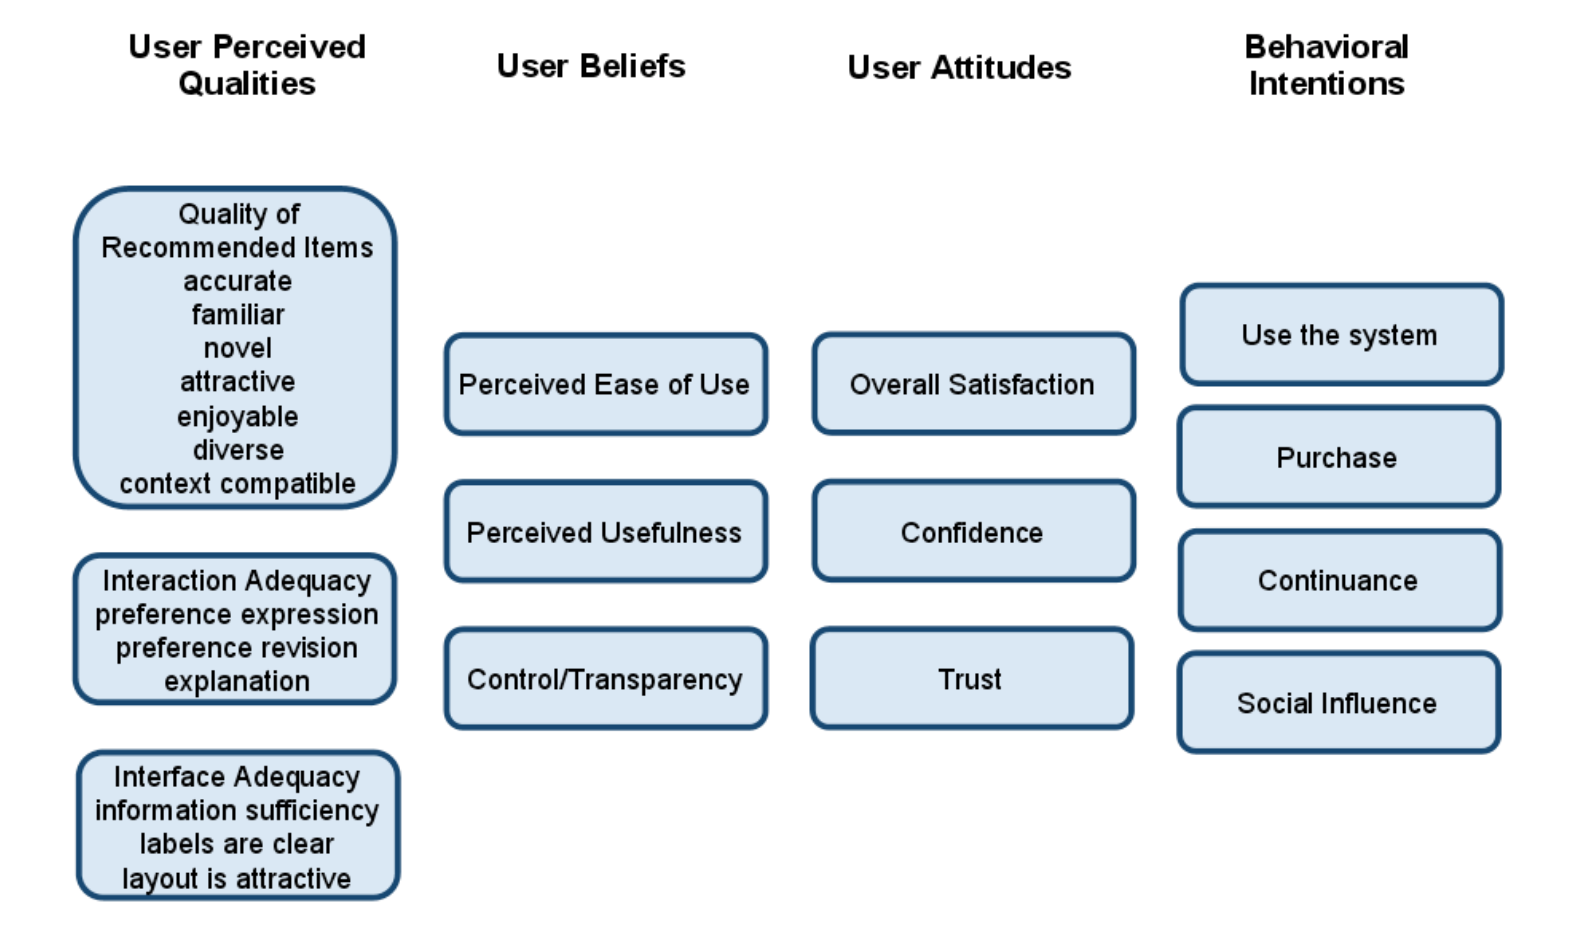
\includegraphics[width=1.2\textwidth]{./Figuras/resque-framework.png}}
  \end{center}
  \legend{Fonte:}
\end{figure}

\section{Apresentação das Recomendações}

No trabalho de Pu et al. (2012) os autores argumentam que apenas a eficiência do algoritmo não garante que o usuário estará satisfeito com o sistema, será leal e continuará utilizando-o ou que os itens serão "convertidos" (nesse sentido, os autores se referem a conversão como a aceitar a recomendação dada e utilizar/comprar/assistir/etc. o item recomendado). Os autores afirmam que percepção do usuário sobre a qualidade da recomendação é afetada tanto pela qualidade das recomendações, que é responsabilidade do algoritmo de recomendação, quanto pela eficiência na apresentação das recomendações, explicando a razão daquelas recomendações e inspirando a confiança do usuário nas suas decisões. Para isso, os autores defendem uma avalição do SR centrada no usuário, de forma a avaliar não somente o algoritmo de recomendação mas o SR como um todo (PU et al., 2012).
Além disso, Pu et al. (2012) definem um conjunto de vinte diretrizes para o design de um SR bem aceito pelos usuários. Essas diretrizes foram criadas a partir da combinação do resultado de vários trabalhos que executaram experimentos com participação de usuários (i.e., Estudos com usuários) para avaliar a interface de SRs. As principais diretrizes levadas em conta por esse trabalho são (PU et al., 2012):

\begin{itemize}
\item Diretriz 14: Considere aprimorar a acurácia percebida pelo usuário com um layout mais atrativo, rótulos mais efetivos, e explicando como o sistema gerou as recomendações. Fazendo isso pode aumentar a percepção do usuário sobre a eficiência do sistema, sua satisfação com o sistema em geral, sua prontidão para aceitar os itens recomendados e a sua confiança no sistema.
\item Diretriz 18: Considere fornecer como recomendação itens compatíveis ao contexto do usuário. Essa característica pode estar altamente relacionada com a percepção de utilidade do sistema e da satisfação do usuário.
\item Diretriz 19: Considere explicar o porquê do sistema recomendou determinados itens. Esses aspectos podem estar altamente relacionados com a satisfação do usuário, a percepção de controle, as intenções do usuário inspiradas pela confiança do usuário, como a intenção de retornar ao sistema.
\item Diretriz 20: Considere fornecer informação suficiente relacionadas aos itens recomendados, controlar a qualidade das informações e da estrutura de navegação.
\end{itemize}

\section{Considerações sobre o capítulo}

\chapter{Trabalhos relacionados}

Todos os trabalhos descritos neste capítulo foram selecionados dentre os artigos analisados no mapeamento sistemático
da literatura \cite{de2017time} sendo considerados aqueles  estão enquadrados dentro da categoria de Decay no que
se refere ao uso do tempo no algoritmo de recomendação, independente do domínio de aplicação. No total oito trabalhos
foram selecionados, sendo apenas um da área educacional.

\section{Fan et al. 2015}

O trabalho de \citeonline{fan2015modeling} realiza a recomendação de web services, considerando a avaliação do serviço
através da medição do Quality of Service (QoS). QoS considera características do serviço como tempo de resposta,
disponibilidade, taxa de serviço, etc. Os autores consideram que a capacidade prever a qualidade de um serviço diminui
conforme o tempo que passou da última invocação desse serviço, devido a possíveis encerramento do serviço, falhas na
rede, etc. Por isso, a recomendação de serviços dos autores combina técnicas de similaridade com uma função de
decaimento que considera que a QoS diminui com o passar do tempo. O modelo de decaimento proposto considera que as
invocações mais recentes de dois usuários a um serviço devem ter um impacto maior no cálculo da similaridade entre os
usuários. O fator de decaimento é calculado utilizando a seguinte fórmula:

\begin{equation}
  \Delta t = \frac{(\Delta t_i + \Delta t_j)}{2}
  \label{eq:fan-fator-decaimento}
\end{equation}


Onde $\Delta t_i$ é o intervalo de tempo entre a invocação do serviço pelo usuário $u_i$ ao serviço e o tempo atual e
$\Delta t_j$ é o intervalo de tempo entre a invocação do mesmo serviço pelo usuário $u_j$ e o tempo atual. Assim, a
similaridade do serviço????  diminui quanto maior for o $\Delta t$. A função de decaimento de um item k é definida como:

\begin{equation}
  f(t_{i,k}, t_{j,k}) = e^{-\alpha \left|t_{atual} - \Delta t \right|}
  \label{eq:fan-funcao-decaimento}
\end{equation}

Onde $\alpha$ é uma constante de decaimento????? . Uma avaliação do serviço é considerada como a combinação do QoS com
a função de decaimento:

\begin{equation}
  r_{u_i, s_k, t} = r_{u_i, s_k} f(t_{i,k}, t_{j,k})
  \label{eq:fan-avaliacao}
\end{equation}

Os autores utilizam a avaliação combinada com a função de decaimento para calcular a similaridade do itens utilizando
um algoritmo chamado PCC????. Que pode ser definido como:

\begin{equation}
  sim(u_1, u_j, t) = \frac{\sum_{s_k \in w_{u_i, u_j}}{(r_{u_i, s_k, t} - \overline{r_{u_i}})(r_{u_j, s_k, t} - \overline{r_{u_j}})}}{\sum_{s_k \in w_{u_i, u_j}}{(r_{u_i, s_k, t} - \overline{r_{u_i}})}^2 \sum_{s_k \in w_{u_i, u_j}}{(r_{u_j, s_k, t} - \overline{r_{u_j}})}^2}
  \label{eq:fan-avaliacao}
\end{equation}


Onde $w_{u_i, u_j}$ é um conjunto dos itens em comum invocados pelos usuários $u_i$ e $u_j$. Utilizando essa fórmula de
similaridade é possível calcular a similaridade entre os usuários e encontrar os que são mais similares.

A proposta dos autores considera também a localização desses usuários para calcular a similaridade. Quanto mais próximos
eles estão, mais similares eles são considerados.

Foi realizado um experimento com o dataset WS-Dream comparando o algoritmo proposto com outros 6 algoritmos. As
métricas utilizadas para a comparação foram MAE e RMSE significado.... Primeiramente foi realizado um experimento
verificando a influência do threshold q???? nos algoritmos. Esse threshold é considerado para decidir quais são os
itens considerados significantes. O segundo experimento avaliou a influência da proporção da base de treino e de teste
no experimento. E por último, para os algoritmos que utilizavam a filtragem colaborativa (o proposto e mais 3) foi
avaliado a influência da quantidade de k-vizinhos considerada na eficiência do algoritmo. Os resultados mostraram que
o algoritmo proposto foi melhor que outros 6 algoritmos analisados.

\section{Luo et al. 2010}

O trabalho de \citeonline{luo2010context} propõe um modelo de recomendação sensível ao contexto para ambientes de
aprendizagem pervasivos. Esse modelo combina uma abordagem híbrida (baseada em conteúdo com filtragem colaborativa)
com uma personalização pelo contexto. Três tipos de contexto são definidos:

\begin{enumerate}
\item Contexto do aluno, que possui as seguintes dimensões: tipo de dispositivo, ambiente (localização), perfil
(informações pessoais como nome e afiliação), preferências (recursos pelo qual o aluno tem interesse), processo de
aprendizagem (histórico de materiais acessados), pedido de acesso (a recursos educacionais massivos).
\item Contexto do serviço, que possui as seguintes dimensões: ambiente (localização), perfil (nome, parâmetros,
retornos), QoS (parâmetros de qualidade do serviço, como carga de trabalho, reputação, disponibilidade, segurança, etc.).
\item Contexto do recurso, que segue o China ELearning Technology Standard que define as dimensões de um recurso
educacional. Esse padrão define as dimensões como sendo: perfil (informações sobre o recurso como Título, Assunto,
Palavras-chave), criador (nome, organização), audiência (tipo de educação, nível de ensino).
\end{enumerate}

O modelo de recomendação proposto pode ser dividido em dois passos: Logic-Based Resource Relevant Degree e
Situation-Based Recourse Relevant Degree.

Na etapa do Logic-based Resource Relevant Degree é feita uma análise o histórico de recursos acessados pelo aluno e as
suas preferências. Esse passo combina a abordagem baseada em conteúdo, filtragem colaborativa e os padrões sequenciais
de acesso.

A abordagem baseada em conteúdo considera as múltiplas dimensões dos recursos como assunto, assunto secundário, nível
de ensino, etc. Nessa abordagem, é inserido um conceito de Preference Energy (PE) para refletir a variação do interesse
do usuário com o passar do tempo. O PE indica que o interesse de um usuário a um item acessado diminui com o passar do
tempo. Os autores definem a diminuição da PE como sendo:

\begin{equation}
  PE_{attenuation}(x) = e^{- \lambda (x-1)}, com \ x \geqslant 1
  \label{eq:luo-preference-energy}
\end{equation}

Onde $x$ é a ordem do recurso na lista de acessos do usuário e $\lambda$ é o parâmetro de decaimento. Esse valor do PE,
combinado com as avalições feitas pelos usuários para os itens são utilizadas para gerar uma Individual Preference Tree
que auxilia o cálculo da similaridade dos recursos candidatos a serem recomendados.

A Individual Preference Tree utilizada pela abordagem baseada em conteúdo também é considerada pelo algoritmo de
filtragem colaborativa definida pelos autores para encontrar os k-vizinhos mais similares. Dessa forma, não só usuários
que acessaram os mesmos itens podem ser considerados vizinhos (como na filtragem colaborativa tradicional), mas também
usuários que acessaram itens similares entre si (mesmo assunto, palavras-chave, etc.) e os avaliaram de forma similar.

O último método de recomendação utilizado pela etapa chamada Logic-based Resource Relevant Degree utiliza os padrões
sequencias de acesso dos usuários aos recursos. O algoritmo utilizado para a mineração dos padrões sequencias é o
PrefixSpan, que procura sequências (ou subsequências) que apareceram em pelo menos  acessos. Baseado na árvore de
padrões sequenciais resultantes do algoritmo de mineração, é calculado quais os itens mais prováveis de serem acessados
de acordo a sequência atual do usuário. A proposta dos autores define que o algoritmo de mineração de sequências deve
ser executado de forma off-line, para garantir a resposta em um tempo hábil.

A etapa de Logic-based Resource Relevant Degree combina o conjunto de recursos recomendados dos três algoritmos
descritos, removendo da lista os recursos já acessados pelo usuário.

Na etapa de Situation-based Resource Relevant Degree é considerado que mesmo um recurso que combine com as preferências
do usuário pode não ser adequados para a recomendação se o contexto do usuário (dispositivo, ambiente) não for adequado
para utilizar o recurso. Para isso, no contexto dos recursos é descrito quais os dispositivos no qual a utilização do
recurso é adequada e no contexto do usuário é descrito qual o dispositivo do usuário. Também é considerado o grau de
satisfação no tempo para acessar um determinado recurso. Isso pode ser calculado pelo tamanho do recurso e a velocidade
de internet do usuário. Combinando essas duas características é possível ter uma recomendação mais adequada a situação
atual do aluno.

O algoritmo de recomendação proposto pelos autores então calcula uma lista de recursos candidatos a recomendação
utilizando os algoritmos de Logic-Based Resource Relevant Degree e remove dessa lista os recursos que não satisfaçam o
dispositivo do usuário e a satisfação mínima com o tempo de resposta esperado.

Esse algoritmo foi avaliado através de uma simulação utilizando o dataset do Movielens, onde foram adicionados dados de
contexto as interações existentes na base. As métricas utilizadas para avaliar o algoritmo foram Precisão, Utilidade e
Validade?????. Em comparação a algoritmos tradicionais de recomendação, o algoritmo proposto teve melhores resultados no
experimento realizado.

\section{Shroff, Dey e Ghosh 2014}

O trabalho de \citeonline{shroff2014enterprise} propõe um modelo para recomendação sensível ao contexto para o ambiente
corporativo. Nesse tipo de ambiente o usuário sobre uma sobrecarga cognitiva, com informações vindo através de redes
sociais, e-mails, noticias, repositórios, etc. O modelo de recomendação busca encontrar poucos itens que tenham uma alta
relevância imediata na tarefa atual do usuário, como por exemplo trocar e-mails com um fornecedor que está com atraso
na entrega ou resolver um problema técnico que um programador esteja encontrando.

As informações para o perfil do usuário são retiradas das mensagens mandadas por este e pelos documentos acessados.
Enquanto os conteúdos são extraídos do twitter, bases de gerenciamento de conhecimento, outros documentos, etc. A
recomendação dos conteúdos leva em conta uma abordagem baseada em conteúdo, combinando com o contexto do usuário.

A abordagem baseada em conteúdo proposta pelos autores utiliza a técnica do TF-IDF em janelas de tempo para identificar
termos de destaque nas ações do usuário, ou seja, termos que aparecem com uma certa frequência em uma janela de tempo
e que não aparece em outras. Isso porque itens que aparecem todo o tempo para determinado usuário devem ser algo do
domínio dele e é considerado pelos autores que não vale a pena ser recomendado.???????

Já a abordagem sensível ao contexto considera a ação atual do usuário, os conceitos presentes nessa ação (por exemplo,
termos presentes no e-mail que usuário escreveu) e a função do usuário (e.g., executivo, vendedor, programador, etc).
Para essa etapa é utiliza uma ontologia das necessidades do usuário que é human-specified, que possui regras do tipo:
ao criar uma proposta mostrar propostas anteriores de sucesso, quando uma entrega estiver atrasada procurar notícias
de eventos que podem ter afetado a entrega. Com base nessa ontologia e nas informações do contexto do usuário o
algoritmo utiliza uma rede bayesiana para o cálculo da probabilidade de cada item ser recomendado.

O algoritmo de recomendação primeiro seleciona os itens utilizando a abordagem baseada em conteúdo para filtrar apenas
os conceitos que podem ser relevantes ao usuário. Depois, os conceitos são ordenados pela probabilidade de serem
relevantes calculada pela rede bayesiana mencionada anteriormente.

Não é realizada uma avaliação do algoritmo de recomendação proposto pelos autores. Eles descrevem cenários e como o
algoritmo iria se portar no cenário com o intuito de demonstrar a utilidade do método.

\section{Benčič e Bieliková 2012}

O sistema de recomendação proposto em \citeonline{bencic2012action} busca recomendar ações aos usuários no momento que
for propício, de acordo com o contexto do usuário, e não apenas quando uma ação do interesse do usuário é encontrada.
Uma ação se refere a qualquer coisa que seja utilizada pelo usuário final de uma aplicação.

O método proposto para a recomendação representa o contexto do usuário através de símbolos, onde cada símbolo de
composto de duas partes – onde uma representa a dimensão e a outra representa a situação particular. Por exemplo,
$Clima:Limpo$. Para cada símbolo do contexto do usuário é atribuído um valor no intervalo $(0, 1)$ que indica a convicção
de que o usuário está naquele contexto.

A convicção de que o usuário está em determinado contexto é observada de tempos em tempos. Esse intervalo depende da
velocidade de conexão do dispositivo do usuário, nível da bateria, etc. A convicção do usuário estar em determinado
contexto diminui com o passar o tempo (supondo que uma nova observação demore a acontecer). Por isso, os autores
utilizam uma função de decaimento para essa convicção conforme a seguir:

\begin{equation}
  CF_t = \frac{CF_b}{(1+r)^t}
  \label{eq:bencic-conviccao}
\end{equation}

Onde $CF_t$ é a convicção calculada em função do tempo $t$, $CF_b$ é a convicção base, $r$ é o fator de decaimento e $t$
é o tempo em horas passado desde a última observação.

As ações são modeladas através de um conjunto de regras. As regras são definidas automaticamente através do feedback do
usuário e são representadas pelos antecedentes (em que situação a regra se aplica) e a consequência (a ação associada
aquela situação). As regras também possuem um decaimento na convicção com o passar o tempo. Porém, nesse caso o
decaimento não constante como para o contexto do usuário. Para as regras o fator de decaimento é calculado de forma
que não aconteça de a maioria das regras chegarem a uma convicção zero se demorar muito para uma nova observação.

Combinando as convicções nas regras criadas com as convicções no contexto do usuário, são encontradas as ações com
maior probabilidade de ser do adequada. O modelo de recomendação considera não apenas a última observação, mas sim uma
combinação das últimas observações e suas respectivas convicções (com o fator de decaimento aplicado).

A avaliação do sistema foi feita realizando simulações de possíveis interações de um usuário imaginário em um ambiente
de recomendação de notícias durante o período de um mês. Nessa simulação foi capturada a convicção de que uma
recomendação de notícias deveria ser realizada para três tipos de usuários: um que lê notícias todos os dias pela
manhã, um que lê notícias apenas nas segundas pela manhã e sextas a noite e outro que começa lendo as notícias apenas
nas segundas pela manhã e muda o seu comportamento com o passar do tempo para a leitura as sextas a noite. Os resultados
mostraram que o método conseguiu compreender o comportamento dos três tipos de usuário com uma precisão e um recall de
quase 100\%.

\section{Hawalah e Fasli 2014}

O trabalho de \citeonline{hawalah2014utilizing} propõe um método de recomendação utilizando o contexto do usuário
representado através de ontologias. O algoritmo proposto pode se adequar a diversos domínios, de forma que o contexto
seja incorporado aos interesses do usuário independente do que são os itens que serão recomendados. Além disso, o método
considera não só o contexto atual do usuário, mas também os contextos capturados anteriormente. Os autores separam o
método em três fases: Extração da informação, Aprender o perfil do usuário e Personalização.

A etapa de Extração da informação é realizada por um agente de captura dos dados que é genérico o suficiente para ser
adaptado de acordo com o domínio. Em determinados domínios pode ser utilizado uma coleta perguntando explicitamente os
interesses e o contexto ao usuário, enquanto em outros domínios é mais adequado capturar de forma implícita pela
navegação do usuário.

A informação bruta capturada (seja de forma explícita ou implícita) é processada pelo agente extrator, responsável por
extrair informação de mais alto nível. Esse agente está associado a dois tipos de bases de conhecimento: ontologias e
taxonomias. O agente realiza um mapeamento os itens que o usuário demonstrou interesse em conceitos da ontologia de
referência, enquanto também extrai dimensões do contexto de mais alto nível utilizando-se das taxonomias de contexto.

A segunda etapa, responsável por compreender o perfil do usuário, utiliza a abordagem de Pré-filtragem Contextual para
definir qual a parte do perfil do usuário é relevante. É utilizada um método similar aos micro-perfis, onde as
informações do perfil do usuário (itens acessados, notas dadas) que aconteceram em contextos similares ao atual são
consideradas mais relevantes para a recomendação. Para isso, é calculado a importância dos conceitos em cada contexto
possível, de acordo com as informações do perfil do usuário. Nesse cálculo, é considerada a frequência com que o
conceito aparece naquele determinado contexto, bem como a frequência com que esse conceito aparece em outros contextos
e a frequência com que outros conceitos aparecem nesse contexto. Detalhes são descritos em \cite{hawalah2014utilizing}.

Ainda no cálculo da importância do conceito em determinado contexto, é considerado que os interesses do usuário podem
mudar com o tempo. Para isso, é incluído na fórmula o fator de Recência (do inglês Recency), de forma que os interesses
demonstrados pelo usuário mais recentemente são considerados mais importantes. A fórmula a seguir é a responsável pelo
cálculo da recência:

\begin{equation}
  Recency(c_j, ce_l) = \frac{1}{(1+\log(d_t - d_l) \times \alpha)}
  \label{eq:hawalah-recencia}
\end{equation}

Onde $d_t$ é a data de inicialização do cálculo, $d_l$ é a data da última ocorrência do conceito $c_j$ no contexto
$ce_l$ e $\alpha$ é o fator de decaimento.

Dessa forma, como resultado dessa etapa temos os interesses do usuário em cada contexto e o peso de cada um. Essas
informações são utilizadas para construir ontologias de perfil contextual personalizada (CPOP, do inglês, contextual
personalized ontology profile), sendo uma CPOP para cada contexto.

Na terceira etapa de personalização, a ontologia gerada na etapa anterior é utilizada para inferir outros conceitos que
o usuário pode ter interesse, além dos já presentes do seu perfil. Isso é realizado utilizando a técnica de Spreading
Activation, descrita em \citeonline{hawalah2014utilizing}. Utilizando essa técnica, é gerada uma lista de recomendações
para cada CPOP, que são combinadas para gerar a lista final de recomendações para o usuário.

A avaliação do trabalho de \citeonline{hawalah2014utilizing} foi um Estudo com Usuários, visando uma avaliação centrada
no usuário como descrito por \citeonline{kelly2009methods}. O objetivo da avaliação era verificar se a recomendação
contextual proposta no trabalho fornece uma recomendação mais eficiente do que os métodos tradicionais. 24 usuários
participaram da avaliação, onde eles utilizaram um sistema por 30 dias, numa estratégia Between-subjects, i.e., cada
grupo testa apenas uma versão do sistema. No total, 4 versões do sistema foram testadas: o algoritmo proposto (CAPS), o
algoritmo proposto sem o uso do contexto (CAPS-C), um método de recomendação personalizado chamado aqui Simple-P e um
método de recomendação não personalizado chamado de Non-P.

O resultado da avaliação analisou a nota dada pelos usuários para os itens em uma escala de likert de 1 a 4. Sendo itens
com grau 1 e 2 considerados uma recomendação ruim e os itens com grau 3 e 4 considerados uma boa recomendação. Com isso
foi possível calcular a Precision at N (P@N). O algoritmo proposto possível o melhor resultado de P@N entre os
algoritmos testados.

\section{Qiao e Zhang 2012}

O trabalho de \citeonline{qiao2015personalized} propõe um algoritmo de recomendação que considera as informações
contextuais disponíveis em dispositivos móveis, como tempo, localização, tipo do dispositivo, etc. O algoritmo de
recomendação é genérico, ou seja, sem um domínio de aplicação definido.

O objetivo dos autores é combinar a filtragem colaborativa com o contexto do usuário, considerando a variação temporal
nos interesses do usuário. Para tal, são encontrados os k usuários com os interesses similares ao usuário atual,
considerando o contexto do usuário, através de técnicas de clusterização. Após encontrados os k vizinhos, utiliza-se
uma fórmula para a predição das notas para itens ainda não acessados pelo usuário com a incorporação de uma função
temporal. A fórmula é a seguinte:

\begin{equation}
  p_{u,i} = \overline{r_u} + \frac{\sum_{v \in U}{sim(u, v)(r_{u,i} - \overline{r_v})f(t_{ni})}}{\sum_{v \in U}{sim(u, v)f(t_{ni})}}
  \label{eq:qiao-predicao}
\end{equation}

Sendo $p_{u,i}$ a nota prevista do usuário $u$ para o item $i$, $\overline{r_u}$ a média das notas dadas pelos usuário
$u$, $sim(u, v)$ a similaridade entre o usuário $u$ e o seu vizinho $v$, $r_{u,i}$ o grau de interesse do usuário $u$
pelo item $i$, $t$ é o tempo no qual o usuário $u$ quer utilizar o item $i$. ?????? Não entendi A função $f$ é a função
exponencial de decaimento que representa a diminuição do interesse do usuário por um determinado item. A função de
decaimento é definida como:

\begin{equation}
  f(t_{ni}) = e^{-t_{ni}}
  \label{eq:qiao-funcao-decaimento}
\end{equation}

Os itens com as notas previstas mais altas são recomendados ao usuário.

A avaliação desse algoritmo foi realizada utilizando a base do MovieLens – 100 K, através da métrica MAE (Erro Absoluto
Médio). Quando comparado a filtragem colaborativa tradicional o algoritmo proposto alcançou melhores resultados, ou
seja, teve uma taxa de erro menor.

\section{Kushwaha et al. 2016}

O trabalho de \citeonline{kushwaha2016inclusion} propõe uma versão modifica da técnica de Joint Matrix Factorization
para uso em um sistema de recomendação de músicas incorporado ao Last.fm. A proposta busca reduzir a esparsidade dos
dados e melhorar a qualidade das recomendações. Para isso, é incorporado informações como descrição dos itens, perfil
do usuário e o seu contexto na matriz das notas dadas pelos Usuários para os Itens comumente utilizada na filtragem
colaborativa. Como a matriz dessa forma possui uma maior dimensionalidade e complexidade, a técnica de fatoração de
matrizes é essencial para reduzir a dimensão desta e permitir a extração de informações latentes importantes para a
recomendação.

Além disso, o algoritmo proposto por \citeonline{kushwaha2016inclusion} considera a variação temporal da informação.
Os autores consideram o decaimento da importância das tags colocadas pelo usuário nos itens com o passar do tempo. A
fórmula utilizada pelos autores para representar o decaimento foi baseada em \citeonline{iofciu2009time}, que pode ser
vista a seguir:

\begin{equation}
  postScore_i = \lambda^{\Delta Time_i}
  \label{eq:kushwaha-funcao-decaimento}
\end{equation}

Onde $postScore_i$ é a importância temporal da tag $i$, $\lambda$ é o fator de decaimento, que deve ser menor do que 1
e foi utilizado por Kushwaha et al. (2016) como 0.9 e $\Delta Time_i$ é o tempo passado desde a interação. Além disso,
é considerada a especificidade da tag para a nota final da tag. A fórmula da especificidade é definida como:

\begin{equation}
  tagSpecificity_i = \log(50+tagCont_i)
  \label{eq:kushwaha-especificidade}
\end{equation}

Onde $tagSpecificity_i$ é o fator de especificidade da tag e $tagCount_i$ representa quanta vezes a tag foi adicionada
ao item $i$. A nota final da tag é:

\begin{equation}
  tagScore_i = \frac{\sum_1^n{postScore}}{tagSpecifity_i}
  \label{eq:kushwaha-nota-final}
\end{equation}

A fórmula acima combina a importância temporal da tag com a sua especificidade. A nota final da tag é incorporada na matriz latente resultado da fatoração de matrizes para servir como fator de decaimento para a importância das tags, representando a variação nos interesses do usuário.
O algoritmo proposto pelos autores foi avaliado utilizando uma base de dados do próprio Last.fm, combinado com a base de dados do DBpedia para a captura de informações sobre os artistas, compositores e músicas. A avaliação considerou a métrica RMSE (root mean square error) para as previsões para as notas que o usuário daria para um determinado item comparada com a nota real. Quando comparado com outros dois algoritmos recentes de recomendação que incorporam informação social para recomendação, o algoritmo proposto por \citeonline{kushwaha2016inclusion} se saiu melhor em 3 das 6 condições de experimento realizadas.

\section{Wei, Khoury e Fong 2013}

\citeonline{wei2013web} descrevem uma proposta de recomendação que utiliza a filtragem colaborativa e que aplica um
decaimento temporal na importância das interações dos usuários. No trabalho, é proposto um serviço para a recomendação
de propagandas em redes sociais, que leva em consideração a confiança entre usuários, a reputação dos usuários e as
relações entre usuários. Os autores afirmam que usuários com uma recomendação gerada com base em usuários conhecidos
pelo usuário atual serão mais bem aceitas, assim como usuários no qual ele confia e nos usuários com alta reputação
(especialistas).

O algoritmo de recomendação considera que a importância da relação entre os usuários diminui gradativamente com o tempo.
Então, um comentário realizado hoje deve ter um peso maior que um comentário realizado ha um mês atrás quando for
avaliada a relação entre dois usuários. O decaimento é incluído diretamente na formula utilizada para realizar a
comparação de similaridade entre dois itens, como pode ser visto a seguir:

\begin{equation}
  s_{i,j}(t) = \frac{\sum_{u \in U_i^t \cap U_j^t}{(f_{ui}^\alpha(t) \cdot r_{ui})(f_{uj}^\alpha(t) \cdot r_{uj})}}{\sqrt{\sum_{u \in U_i^t}{(f_{ui}^\alpha(t) \cdot r_{ui})}^2 \sum_{u \in U_j^t}{(f_{uj}^\alpha(t) \cdot r_{uj})}^2}}
  \label{eq:wei-similaridade}
\end{equation}

Onde a função $f$ é definida pelos autores como relevância temporal do item e pode ser vista como:

\begin{equation}
  f_{uj}^\alpha(t) = e^{- \alpha (t - t_{ui})}
  \label{eq:wei-relevancia-temporal}
\end{equation}

Onde fator $\alpha$ é responsável por controlar a taxa de decaimento, $t$ representa o tempo atual e $t_{ui}$ representa
o tempo no qual o usuário $u$ utilizou o item $i$.

Além do decaimento na relevância das relações entre os usuários, os autores também incluem a confiança entre os
usuários e a reputação de especialistas da área na formula de similaridade visando melhorar a qualidade das
recomendações.

O algoritmo proposto foi avaliado utilizando três bases de dados: MovieLens, Facebook e Delicious. O algoritmo foi
comparado a outros dois algoritmos: Filtragem Colaborativa usando correlação de Pearson e usando correlação de Pearson
com efeito temporal. As métricas utilizadas foram Mean Absolute Error e Root Mean Square Deviation. Os resultados
mostraram que o algoritmo proposto melhorou significativamente a qualidade das recomendações.

\section{Considerações sobre o capítulo}

\chapter{SR Sensível ao Tempo}\label{chapter:proposta}

Neste capítulo é apresentado o SR Sensível ao Tempo para ambientes educacionais proposto nesse trabalho. O algoritmo proposto
considera o decaimento nos interesses do usuário com o passar do tempo (categoria do \textit{Decay} - Seção \ref{section:decay}). Nesse capítulo é apresentado
o algoritmo proposto, uma análise das suas vantagens e cenários que ilustram o uso desse algoritmo.

\section{Algoritmo Proposto}\label{section:algoritmo-proposto}

O algoritmo de recomendação proposto nesse trabalho combina a Abordagem Baseada em Conteúdo tradicional com o uso do
contexto temporal através da categoria \textit{Decay} (ver seção \ref{section:decay}).

O cálculo da relevância de um determinado item $i$ para um usuário $u$ no algoritmo proposto está formalizada na Equação
\ref{eq:relevancia-proposta}.

\begin{equation}
  F(u,i) = S(u,i) \cdot R(I_{u,i}) + A(i)
  \label{eq:relevancia-proposta}
\end{equation}

Onde: $F$ é a função que calcula a relevância de um item $i$ para um usuário $u$; $S$ é a função de similaridade entre
o perfil do usuário $u$ (representado através de conjunto de palavras-chave dos itens acessados) e o item $i$
(representado pelo conjunto de palavras-chave que o caracterizam); $R$ é o maior valor de recência dos itens do conjunto
$I_{u,i}$ (itens acessados pelo usuário $u$ e com alguma similaridade com o item $i$); $A$ é uma função que retorna $1$
se o item $i$ nunca foi acessado pelo usuário u e $0$ se o item já foi acessado.

A função $S$ de similaridade entre o usuário $u$ e o item $i$ é calculada utilizando a fórmula do cosseno (ver Seção
\ref{subsection:baseada-em-conteudo}). A função de recência $R$, responsável pelo \textit{Decay}, estéa definida na Equação
\ref{eq:recencia-proposta}.

\begin{equation}
  R(I_{u,i}) = \max_{\{j \in I_{u,i}\}}{\frac{x_j}{\left| I_u \right|}}
  \label{eq:recencia-proposta}
\end{equation}

Onde: $x_j$ é a posição do item j na lista de itens acessados pelo usuário $u$ ordenada de forma crescente pelo
\textit{timestamp} do acesso; e $\left| I_u \right|$ é a quantidade de itens acessados pelo usuário $u$. Essa fórmula considera
que mais de um item acessado pelo usuário pode ser similar ao item $i$, por isso a fórmula retorna a maior recência de
todos os itens presentes no perfil do usuário que são similares a $i$. A seguir temos um exemplo do uso da fórmula da
recência de um item, que pode ser estendida para o uso com vários itens e aplicada a função $max$ como descrito na
fórmula acima.

Considerando um usuário $u$ que acessou três itens diferentes nos seguintes \textit{timestamps} (em \textit{epoch}):
Item A acessado $1503670382$; Item B acessado em $1500027182$; Item C acessado em $1508051582$. Ao ordenar esses itens
pelo \textit{timestamp}, em ordem crescente, temos: (1) Item B, (2) Item A, (3) Item C. As equações \ref{eq:recencia-item-a},
\ref{eq:recencia-item-b} e \ref{eq:recencia-item-c} apresentam o resultado do cálculo de recência para cada um dos itens:

\begin{equation}
  R(A) = \frac{2}{3} = 0.\overline{6}
  \label{eq:recencia-item-a}
\end{equation}

\begin{equation}
  R(B) = \frac{1}{3} = 0.\overline{3}
  \label{eq:recencia-item-b}
\end{equation}

\begin{equation}
  R(C) = \frac{3}{3} = 1.0
  \label{eq:recencia-item-c}
\end{equation}

No Algoritmo \ref{alg:proposta-pseudocodigo} é possível observar o pseudo-código do algoritmo proposto. Nesse algoritmo
está representado em mais alto nível as etapas da recomendação. Primeiramente, são buscados no banco de dados a lista de itens
acessados pelo usuário e a lista de itens que podem ser recomendados. O cálculo da recência para cada item do perfil do usuário
é feito também na fase de inicialização, pois esse cálculo só precisa ser realizado uma vez. Depois disso, para cada item
candidato a ser recomendado para o usuário, é calculada a similaridade do perfil do usuário (composto pelas palavras dos itens acessados
por ele) com as palavras-chave do item candidato. Nessa etapa também é encontrado qual o item do perfil do usuário que é semelhante
ao item candidato e é mais recente, para utilizar o seu valor de recência no cálculo do score.

\begin{algorithm}\label{alg:proposta-pseudocodigo}
  \caption{Pseudo-código do Algoritmo de Recomendação Proposto}

  \SetKwInOut{Input}{input}
  \SetKwInOut{Output}{output}
  \SetKwProg{algoritmoRecomendacaoDecay}{algoritmoRecomendacaoDecay}{}{}

  \algoritmoRecomendacaoDecay{$(Usuário)$}{
    \Input{Usuário que irá receber a recomendação.}
    \Output{Lista com cinco itens recomendados para o usuário.}
    itens = buscarItensCandidatos()\;
    itensPerfilUsuario = buscarItensPerfil(Usuário)\;


    recênciaItensPerfil = calcularRecência(itensPerfilUsuario)\;
    scores = \{\}\;

    \ForEach{$item \in itens$}{
      similaridade, itensSimilares = calcularCosseno(itensPerfilUsuario, item)\;
      recência = calcularMaxRecência(itensSimilares, recênciaItensPerfil)\;
      scores[item] = similaridade * recência + item.acessado\;
    }

    \Return scores.max(5)\;
  }
\end{algorithm}

O cálculo do score para o item candidato é finalmente realizado utilizando a Equação \ref{eq:relevancia-proposta}. Os cinco
itens com o maior score são retornados pelo algoritmo para serem recomendados ao usuário.

No Algoritmo \ref{alg:calcular-recencia-pseudocodigo} é demonstrado o cálculo da recência para cada um dos itens do perfil do
usuário, que é utilizado pelo Algoritmo \ref{alg:proposta-pseudocodigo} descrito anteriormente. Nesse cálculo, os itens são
ordenados pela data de acesso inicialmente e após isso uma versão simplificada da Equação \ref{eq:recencia-proposta} é aplicada.
A função $max$ presente na Equação \ref{eq:recencia-proposta} não é aplicada nesse momento, sendo cálculada apenas a recência
para cada item individualmente. No método descrito no Algoritmo \ref{{alg:calcular-recencia-pseudocodigo}} é que será aplicado
o $max$ nas recências, para encontrar a maior recência entre os itens similares ao item candidato à recomendação.

\begin{algorithm}
  \caption{Pseudo-código do cálculo da recência para cada item presente no perfil do usuário \label{alg:calcular-recencia-pseudocodigo}}

  \SetKwInOut{Input}{input}
  \SetKwInOut{Output}{output}
  \SetKwProg{calcularRecencia}{calcularRecência}{}{}

  \calcularRecencia{$(itensPerfilUsuario)$}{
    \Input{Lista de itens acessados pelo usuário.}
    \Output{Hash com a recência calculada para cada item no perfil do usuário.}
    recênciaItensPerfil = \{\}\;
    itensOrdenados = itensPerfilUsuario.ordenarPor(dataAcesso)\;
    tamanhoPerfilUsuario = itensPerfilUsuario.tamanho()\;

    \ForEach{$item \in itensPerfilUsuario$}{
      recênciaItensPerfil[item] = itensOrdernados.find(item).posição() / tamanhoPerfilUsuario\;
    }

    \Return recênciaItensPerfil\;
  }
\end{algorithm}

\begin{algorithm}\label{alg:max-recencia-pseudocodigo}
  \caption{Pseudo-código do cálculo da recência máxima entre os itens do perfil do usuário similares ao item candidato}

  \SetKwInOut{Input}{input}
  \SetKwInOut{Output}{output}
  \SetKwProg{calcularMaxRecencia}{calcularMaxRecência}{}{}

  \calcularMaxRecencia{$(itensSimilares, recênciaItensPerfil)$}{
    \Input{Lista de itens similares e hash com a recência calculada para cada item do perfil do usuário.}
    \Output{Valor máximo de recência entre itens similares.}

    recênciaItensSimilares = recênciaItensPerfil.find(itensSimilares)\;

    \Return recênciaItensSimilares.max(1)\;
  }
\end{algorithm}


\section{Discussão Sobre o Algoritmo Proposto}

Um ponto negativo da Filtragem Colaborativa é a necessidade de uma comunidade de usuários ativa, que nem sempre é
possível em um AVA onde as turmas muitas vezes são menores (entre 10 e 100 alunos). A Abordagem Baseada
em Conteúdo é considerada para o SR porque essa abordagem permite a recomendação em um sistema que não possui uma
comunidade ativa e pode suprir as necessidades desse domínio.

Os SRs Sensíveis ao Tempo tem uma vantagem em relação à outros SRs Sensíveis ao Contexto por a informação temporal ser
mais simples de capturar e manipular que outras informações contextuais, e.g., localização. Além disso, esses tipos de
algoritmos estão sendo explorados em outros domínios de aplicação, como pode ser visto nos 88 artigos analisados no
Mapeamento Sistemático realizado \cite{de2017time}, e demonstraram bons resultados. Por isso, esse trabalho busca
aplicar o contexto temporal no algoritmo de recomendação na área educacional (na qual foram encontrados apenas quatro
trabalhos) e avaliar os resultados.

A escolha do \textit{Decay} se justifica como forma de procurar minimizar uma das grandes desvantagens da abordagem Baseada em Conteúdo: a
Superespecialização. Na abordagem Baseada em Conteúdo as recomendações seriam geradas levando em conta todos os itens
acessados pelo usuário igualitariamente. Enquanto ao aplicar o \textit{Decay}, os itens acessados mais recentemente possuem um
grau de importância maior para o algoritmo do que itens acessados anteriormente. Dessa forma, mesmo que o usuário
tenha acessado muitos materiais sobre determinado assunto, ao começar a acessar materiais sobre outro assunto o algoritmo de
recomendação consegue rapidamente se adaptar e gerar recomendações sobre esse novo conteúdo.

Um cenário de uso do \textit{Decay} é apresentado a seguir. \textit{O aluno Pedro está matriculado em uma disciplina de Estrutura de Dados
que possui quatro tópicos, sendo eles Pilhas, Filas, Listas e Árvores. Nessa disciplina, para cada um dos conteúdos é
aplicada uma prova para avaliar os conhecimentos dos alunos. Até o momento da primeira prova sobre o conteúdo de Pilhas,
Pedro acessou apenas materiais relacionados a Pilhas. O algoritmo de recomendação utilizando a abordagem Baseada em
Conteúdo recomenda para Pedro apenas materiais relacionados a Pilhas. Após a primeira prova, Pedro começa a acessar
materiais relacionados a Filas, o segundo tópico da disciplina. Em uma abordagem Baseada em Conteúdo tradicional as
recomendações continuariam sendo sobre o conteúdo de Pilhas por um bom tempo, pois o perfil de Pedro seria em grande
parte composto por materiais acessados sobre esse assunto. Porém, com o uso do \textbf{Decay}, no momento em que Pedro começar a
acessar materiais sobre Filas o algoritmo de recomendação dará um peso maior para esses materiais (sem ignorar os itens
acessados anteriormente) e em pouco tempo Pedro já estará recebendo recomendações sobre o novo tópico estudado. Da mesma
forma, se Pedro voltar a acessar conteúdos anteriores para relembrar algum conceito, o SR também perceberá isso e
recomendará itens relacionados ao primeiro conteúdo novamente.}

O algoritmo proposto nesse trabalho considera o decaimento no peso dos itens do perfil do usuário em função da posição
do item na sequência de materiais acessados, como mostrado na Seção \ref{section:algoritmo-proposto}, e não na quantidade de tempo passada em
segundos como feito na maioria dos trabalhos relacionados mostrados no Capítulo \ref{chapter:trabalhos-relacionados}. Isso é uma vantagem, pois no domínio
educacional o passar do tempo não é tão relevante quanto em outros domínios, como na recomendação de \textit{Web Services} por
exemplo.

Os alunos em um AVA podem ter ritmos de estudo diferentes e, por isso, é assumido nesse trabalho que faz
mais sentido analisar quantos itens foram acessados desde do acesso de determinado material do que o tempo passado desde
a interação. Dessa forma, esse algoritmo não considera se o usuário acessou todos os itens do seu perfil em um
único dia, ou se ele acessou metade do materiais na primeira semana do curso e a outra metade na última semana ou se ele
acessou alguns materiais todos os dias durante o curso.

Além disso, no algoritmo proposto nesse trabalho não é definido um fator de decaimento único para os todos os usuários como nos trabalhos
relacionados apresentados no Capítulo \ref{chapter:trabalhos-relacionados}. Isto porque é necessário considerar
que cada aluno tem um estilo de aprendizagem diferente e o decaimento para um aluno poderia ser diferente do decaimento
para outros alunos. E não foram encontrados nos trabalhos relacionados que mostrem um modelo para calcular o fator de decaimento de forma
personalizada para cada usuário. Em geral, os autores utilizam o fator de decaimento escolhido de forma empírica e
aplicam o mesmo fator para todos os usuários.

\section{Considerações sobre o capítulo}

Nesse capítulo é apresentada a proposta desse trabalho. O algoritmo proposto utiliza a abordagem Baseada em Conteúdo em
conjunto com o uso do tempo através da categoria \textit{Decay}, ou seja, é dado um peso menor na recomendação para os
itens acessados a mais tempo pelo usuário e um peso maior para os itens mais recentes. No Sistema de Recomendação (SR)
proposto é combinada a similaridade entre o perfil do usuário e os itens, a recência dos itens acessados pelo usuário e
se os links recomendados já foram ou não acessados. O algoritmo proposto será avaliado utilizando o experimento descrito
no Capítulo \ref{chapter:experimento}



\chapter{Planejamento do Experimento}

\section{Definição do experimento}

\section{Minicurso de Algoritmos}

\section{Desenvolvimento dos instrumentos}

\section{Teste piloto}

\section{Considerações sobre o capítulo}

\chapter{Conclusões}\label{chapter:conclusoes}


% ---
% Finaliza o bookmark do PDF
% ---
\bookmarksetup{startatroot}%
% ---

% ----------------------------------------------------------
% ELEMENTOS PÓS-TEXTUAIS
% ----------------------------------------------------------
\postextual

% ----------------------------------------------------------
% Referências bibliográficas
% ----------------------------------------------------------
\bibliography{references}

% ----------------------------------------------------------
% Glossário
% ----------------------------------------------------------
%
% Consulte o manual da classe abntex2 para orientações sobre o glossário.
%
%\glossary

% ----------------------------------------------------------
% Apêndices
% ----------------------------------------------------------
\begin{apendicesenv}
  % Imprime uma página indicando o início dos apêndices
  \partapendices

  \chapter{Cronograma das atividades}\label{cha:cronograma}

Este apêndice apresenta o cronograma das atividades durante todo o desenvolvimento dessa pesquisa e das etapas que ainda
estão por vir. Cada atividade está numerada no cronograma e explicada em detalhe abaixo.

\begin{figure}[htb]
  \begin{center}
      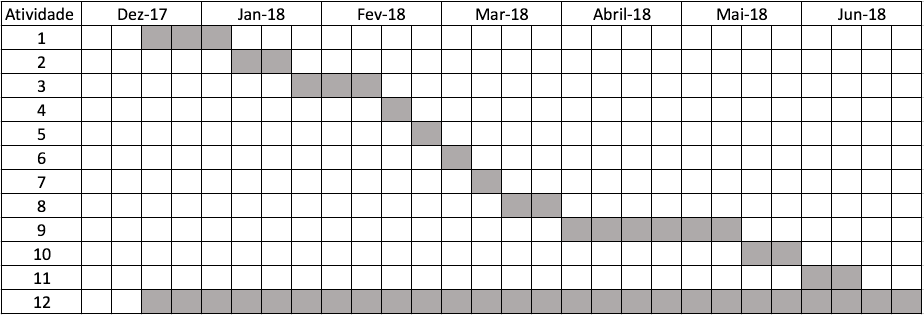
\includegraphics[scale=0.5]{./Figuras/cronograma.png}
  \end{center}
  \legend{Fonte: \citeonline{gasparini2003interface}}
\end{figure}

\begin{enumerate}
\item Estudo dos Sistemas de Recomendação aplicados em Ambientes Virtuais de Aprendizagem
\item Estudo dos Sistemas de Recomendação Sensíveis ao Tempo
\item Análise de como aplicar os Sistemas de Recomendação Sensíveis ao Tempo em Ambientes Virtuais de Aprendizagem
\item Estudo das formas de avaliação de Sistema de Recomendação
\item Estudo das métricas para avaliação de Sistemas de Recomendação
\item Estudo das formas de avaliação de Sistema de Recomendação em Ambientes Virtuais de Aprendizagem
\item Identificar as características do AdaptWeb\textsuperscript{\textregistered}
\item Estudo para decidir o algoritmo a ser utilizado
\item Identificar os pontos de alteração no AdaptWeb\textsuperscript{\textregistered}
\item Definir a forma de avaliação a ser realizada e as métricas utilizadas
\item Implementar a proposta no AdaptWeb\textsuperscript{\textregistered}
\item Realizar o experimento para avaliação da proposta
\item Analisar os resultados do experimento
\item Escrever a dissertação
\end{enumerate}

\end{apendicesenv}

% ----------------------------------------------------------
% Anexos
% ----------------------------------------------------------
\begin{anexosenv}
  % Imprime uma página indicando o início dos anexos
  \partanexos

  % ---
\chapter{60 Questões do Framework de Avaliação de Sistemas de Recomendação ResQue}\label{ane:questoes-framework}
% ---
\lipsum[30]

% ---
\chapter{Cras non urna sed feugiat cum sociis natoque penatibus et magnis dis
parturient montes nascetur ridiculus mus}
% ---

\lipsum[31]

% ---
\chapter{Fusce facilisis lacinia dui}
% ---

\lipsum[32]
\end{anexosenv}

\end{document}